\documentclass{article}

\usepackage[utf8]{inputenc}
\usepackage[T1]{fontenc}
\usepackage[francais]{babel}
\usepackage{titling}
\setlength{\droptitle}{-3cm}
\usepackage{graphicx}
\usepackage{underscore}
\usepackage{hyperref} 
\usepackage{wrapfig}


\title{Visualisations, graphiques}
\author{CAROT Axel, ARISOY Ivan Can}
\date{\today}

\begin{document}
\maketitle

\section{Analyses descriptives}
Nous avons commencé par réaliser différentes visualisations descriptives sur une partie de nos données : "corpusbf.xlsx". Ce corpus contient des informations sur les articles qui ne sont pas forcément présentes dans le reste de nos données, telles que : VOC_SA, VOC_CR, ANNEE ou encore NEG (indice de négativité développé par nos commanditaires).

\begin{figure}[h]
    \centering
    \begin{minipage}{.45\textwidth}
        \centering
        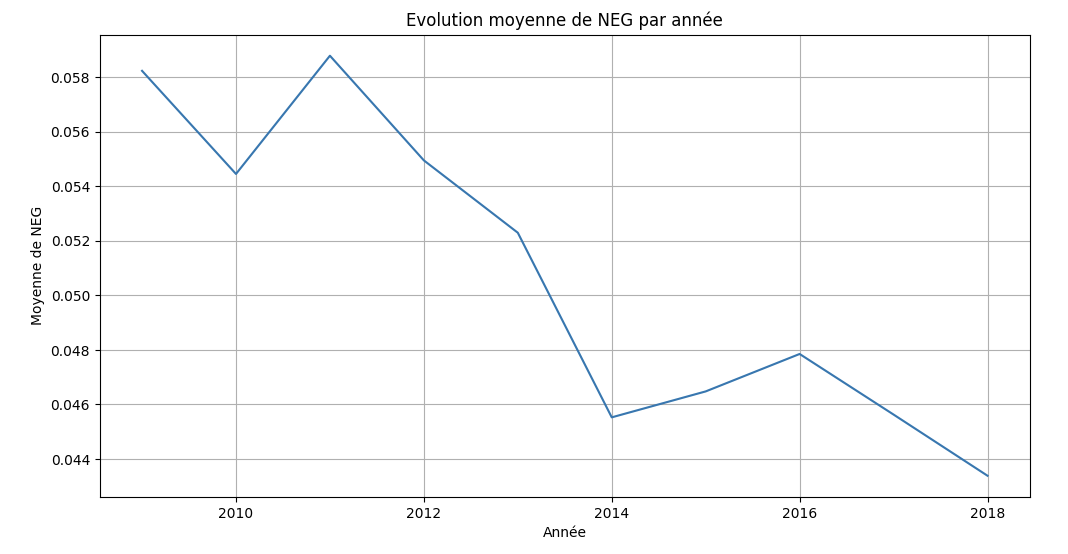
\includegraphics[width=0.9\linewidth]{evol_neg.png}
        \caption{Evolution moyenne de \\l'indice de négativité par année}
        \label{fig:Evolution moyenne de l'indice de négativité par année}
    \end{minipage}%
    \begin{minipage}{.5\textwidth}
        \centering
        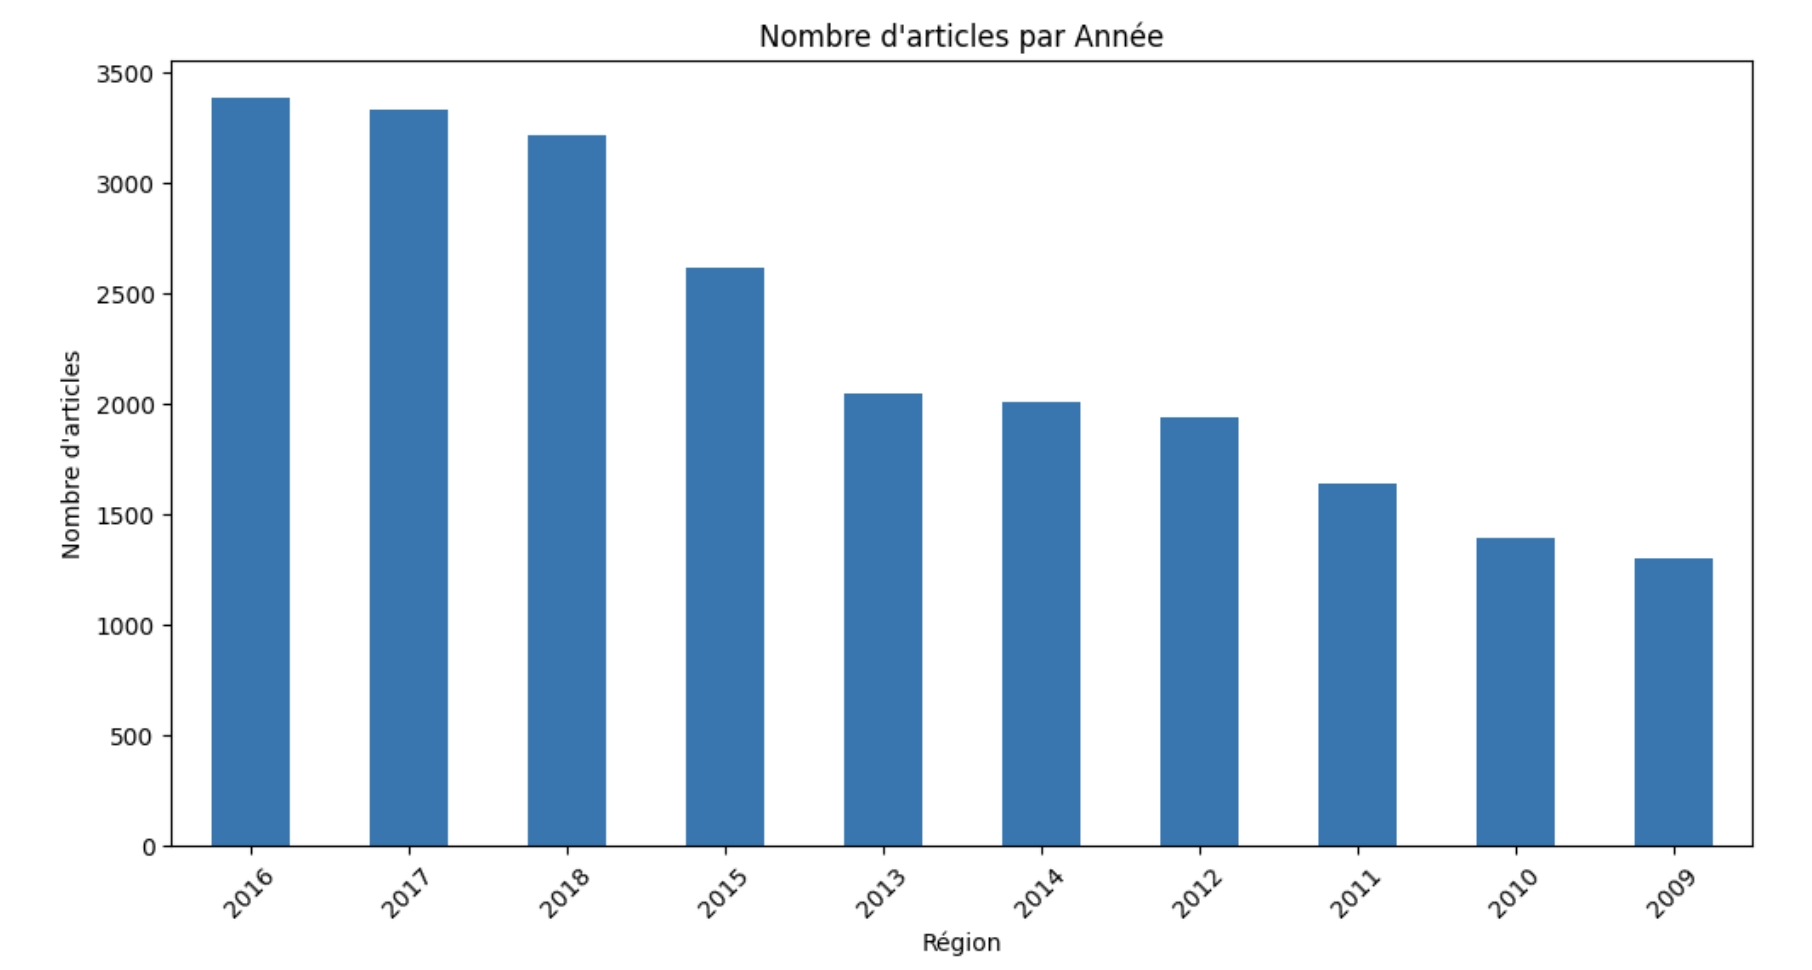
\includegraphics[width=0.9\linewidth]{nb_article_annee.png}
        \caption{Nombre d'articles par année}
        \label{fig:Nombre d'articles par année}
    \end{minipage}
\end{figure}

En utilisant ces variables, nous pouvons observer que les années où nous disposons du plus grand nombre d'articles se situent entre 2016 et 2018. L'indice de négativité présente une tendance à la baisse au fil des années.

\begin{figure}[h]
    \centering
    \begin{minipage}{.5\textwidth}
        \centering
        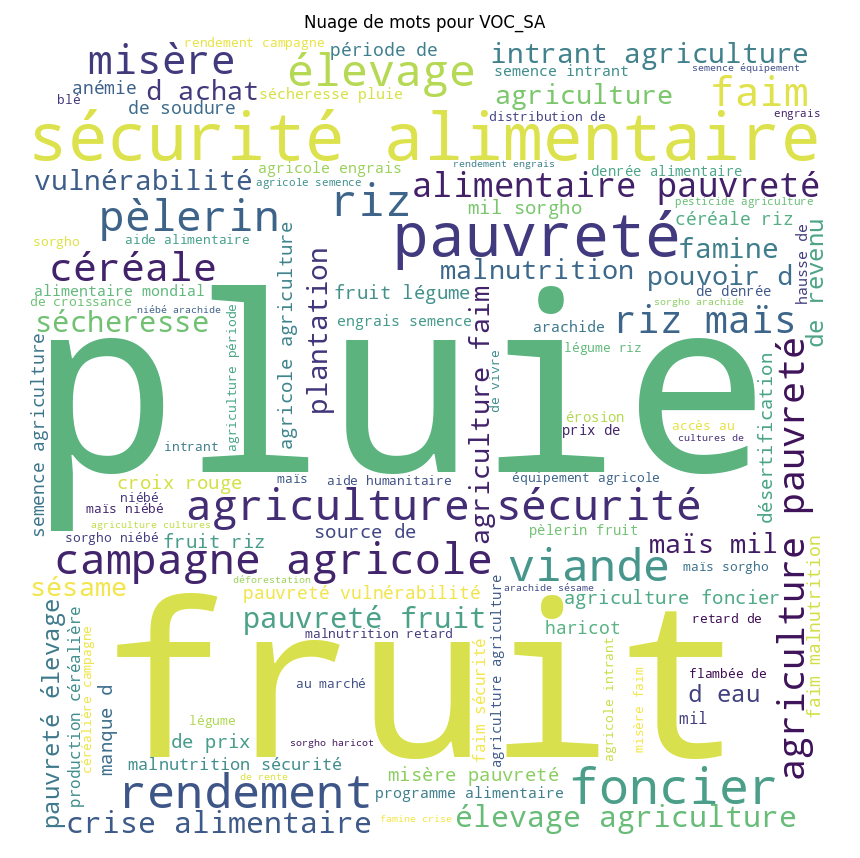
\includegraphics[width=0.8\linewidth]{nuage_ca.png}
        \caption{Nuage de mot pour \\VOC_SA}
        \label{fig: Nuage de mot pour VOC_SA}
    \end{minipage}%
    \begin{minipage}{.5\textwidth}
        \centering
        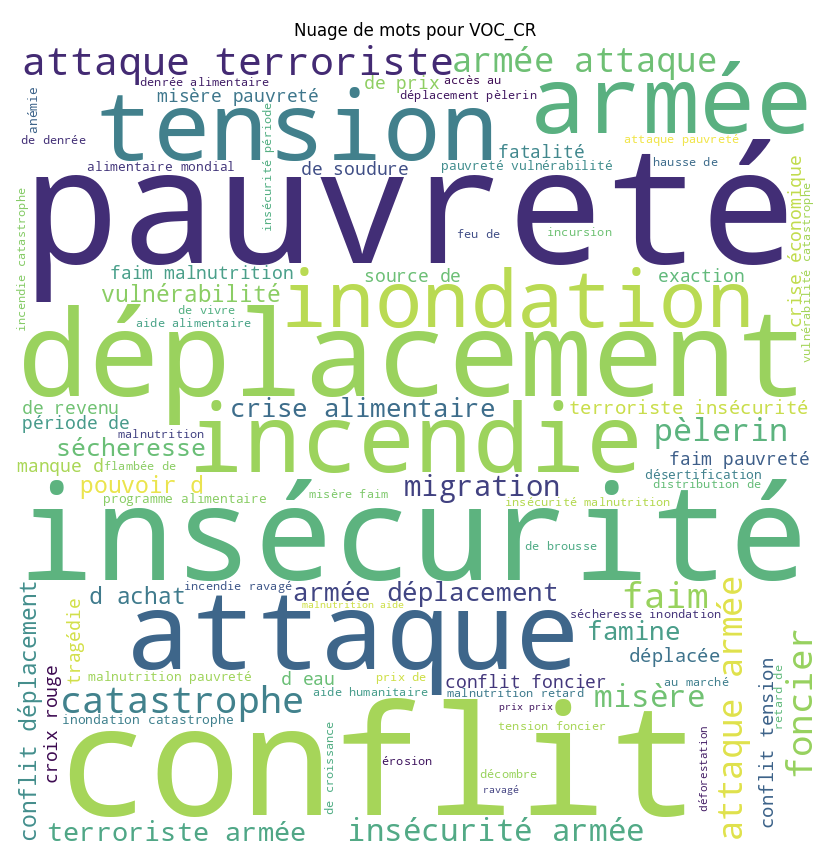
\includegraphics[width=0.8\linewidth]{nuage_cr.png}
        \caption{Nuage de mot pour \\VOC_CR}
        \label{fig: Nuage de mot pour VOC_CR}
    \end{minipage}
\end{figure}

Nous disposons également, pour chaque article, de deux variables répertoriant les mots-clés liés à la sécurité alimentaire présents dans les textes. Les listes initiales de mots-clés ont été rédigées par nos commanditaires ainsi que par des spécialistes. Ces nuages de points permettent d'identifier les mots-clés les plus fréquemment présents dans les textes.

\section{Développement et Fine-tuning du Modèle BERT à l'Aide de WandB}

\subsection{Weights and Biases}

\begin{wrapfigure}{r}{0.25\textwidth} % "r" pour droite, et la largeur de l'enveloppe
  \centering
  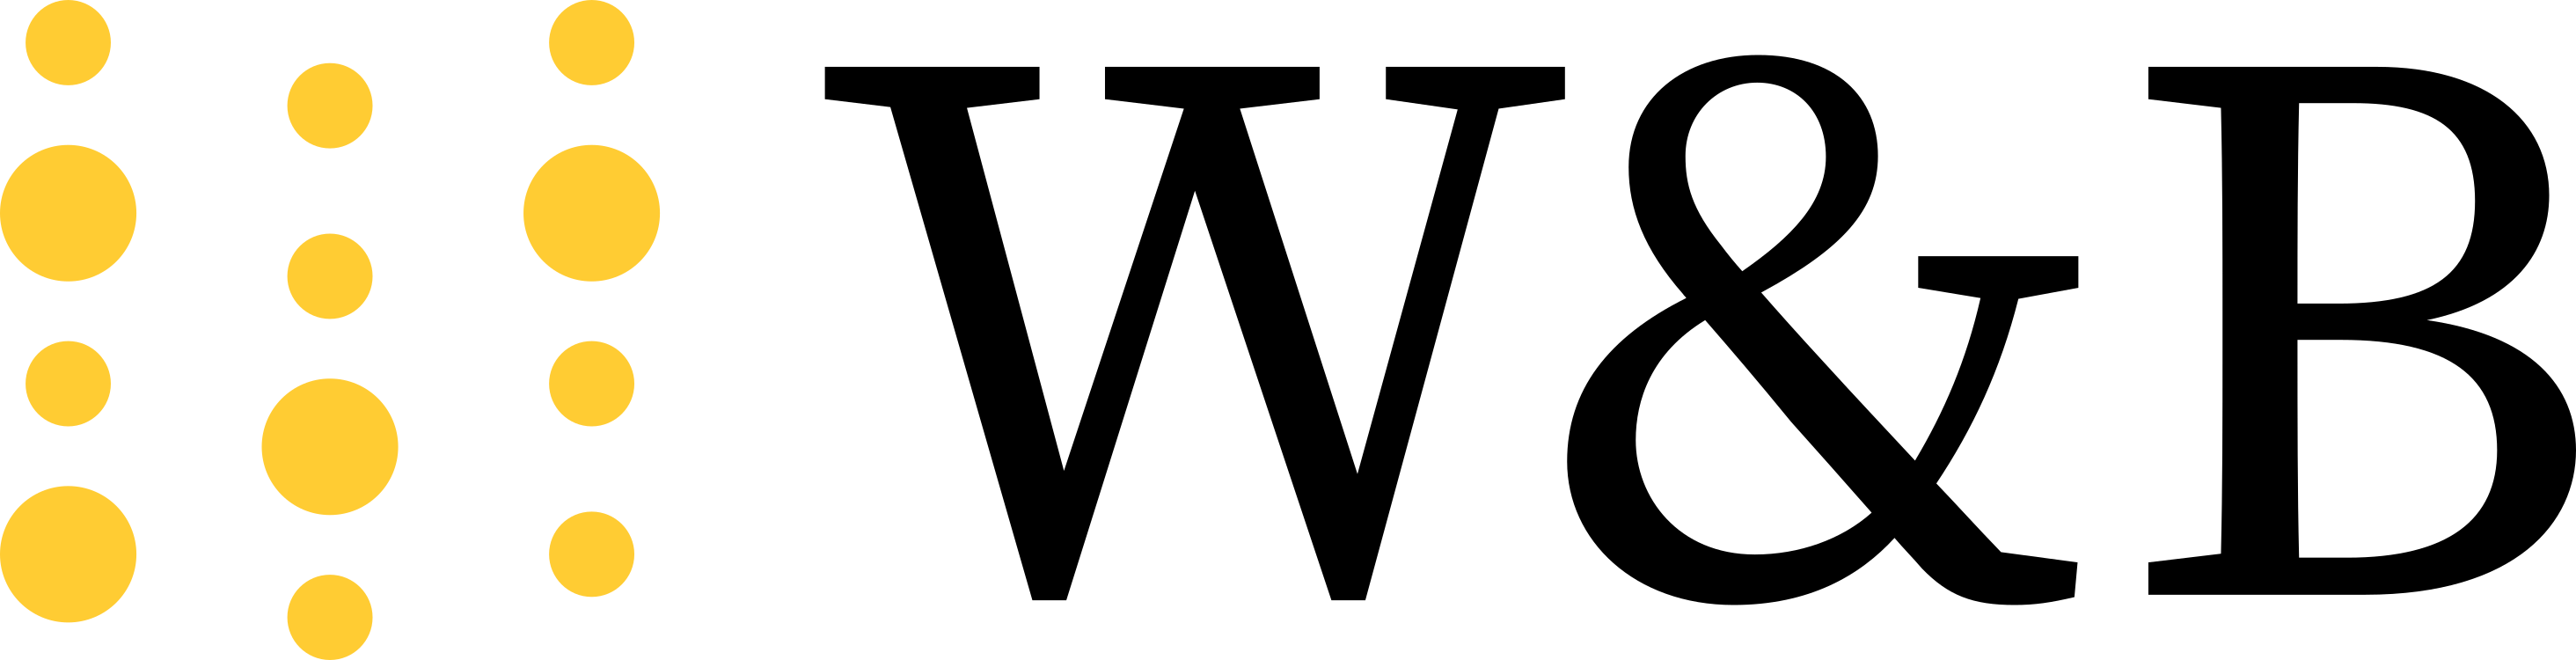
\includegraphics[width=0.2\textwidth]{image.png}
  \caption{\small Weights and Biases}
  \label{fig:Weights and Biases}
\end{wrapfigure}

Pour le développement de notre modèle de pertinence, nous avons opté pour une approche Nested K-Fold Cross Validation combinée à une recherche exhaustive afin de fine-tuner nos hyperparamètres. Puisque que cette approche est longue et coûteuse, Weights and Biases (WandB), un outil de suivi et d'optimisation d'apprentissage automatique, nous aide à conserver toutes les métriques tout au long du développement. Il offre la possibilité de suivre les recherches des combinaisons d'hyperparamètres à l'aide des fonctionnalités "sweep", ce qui est très pertinent pour notre cas.

\subsection{Interprétation des Résultats}

Le système de dashboard de WandB permet une visualisation claire des évolutions et des performances d'apprentissage et facilite l'exportation de ces informations. L'application de la Nested K-Fold Cross Validation avec les sweeps d'hyperparamètres nous permet de suivre et de choisir la meilleure combinaison d'hyperparamètres pour le modèle. Cette approche est cruciale dans le contexte de notre projet car nous disposons d'un jeu de données étiquetées relativement petit et nous devons à la fois identifier les hyperparamètres optimaux et évaluer la capacité de généralisation du modèle.

\begin{figure}[!htbp]
    \centering
    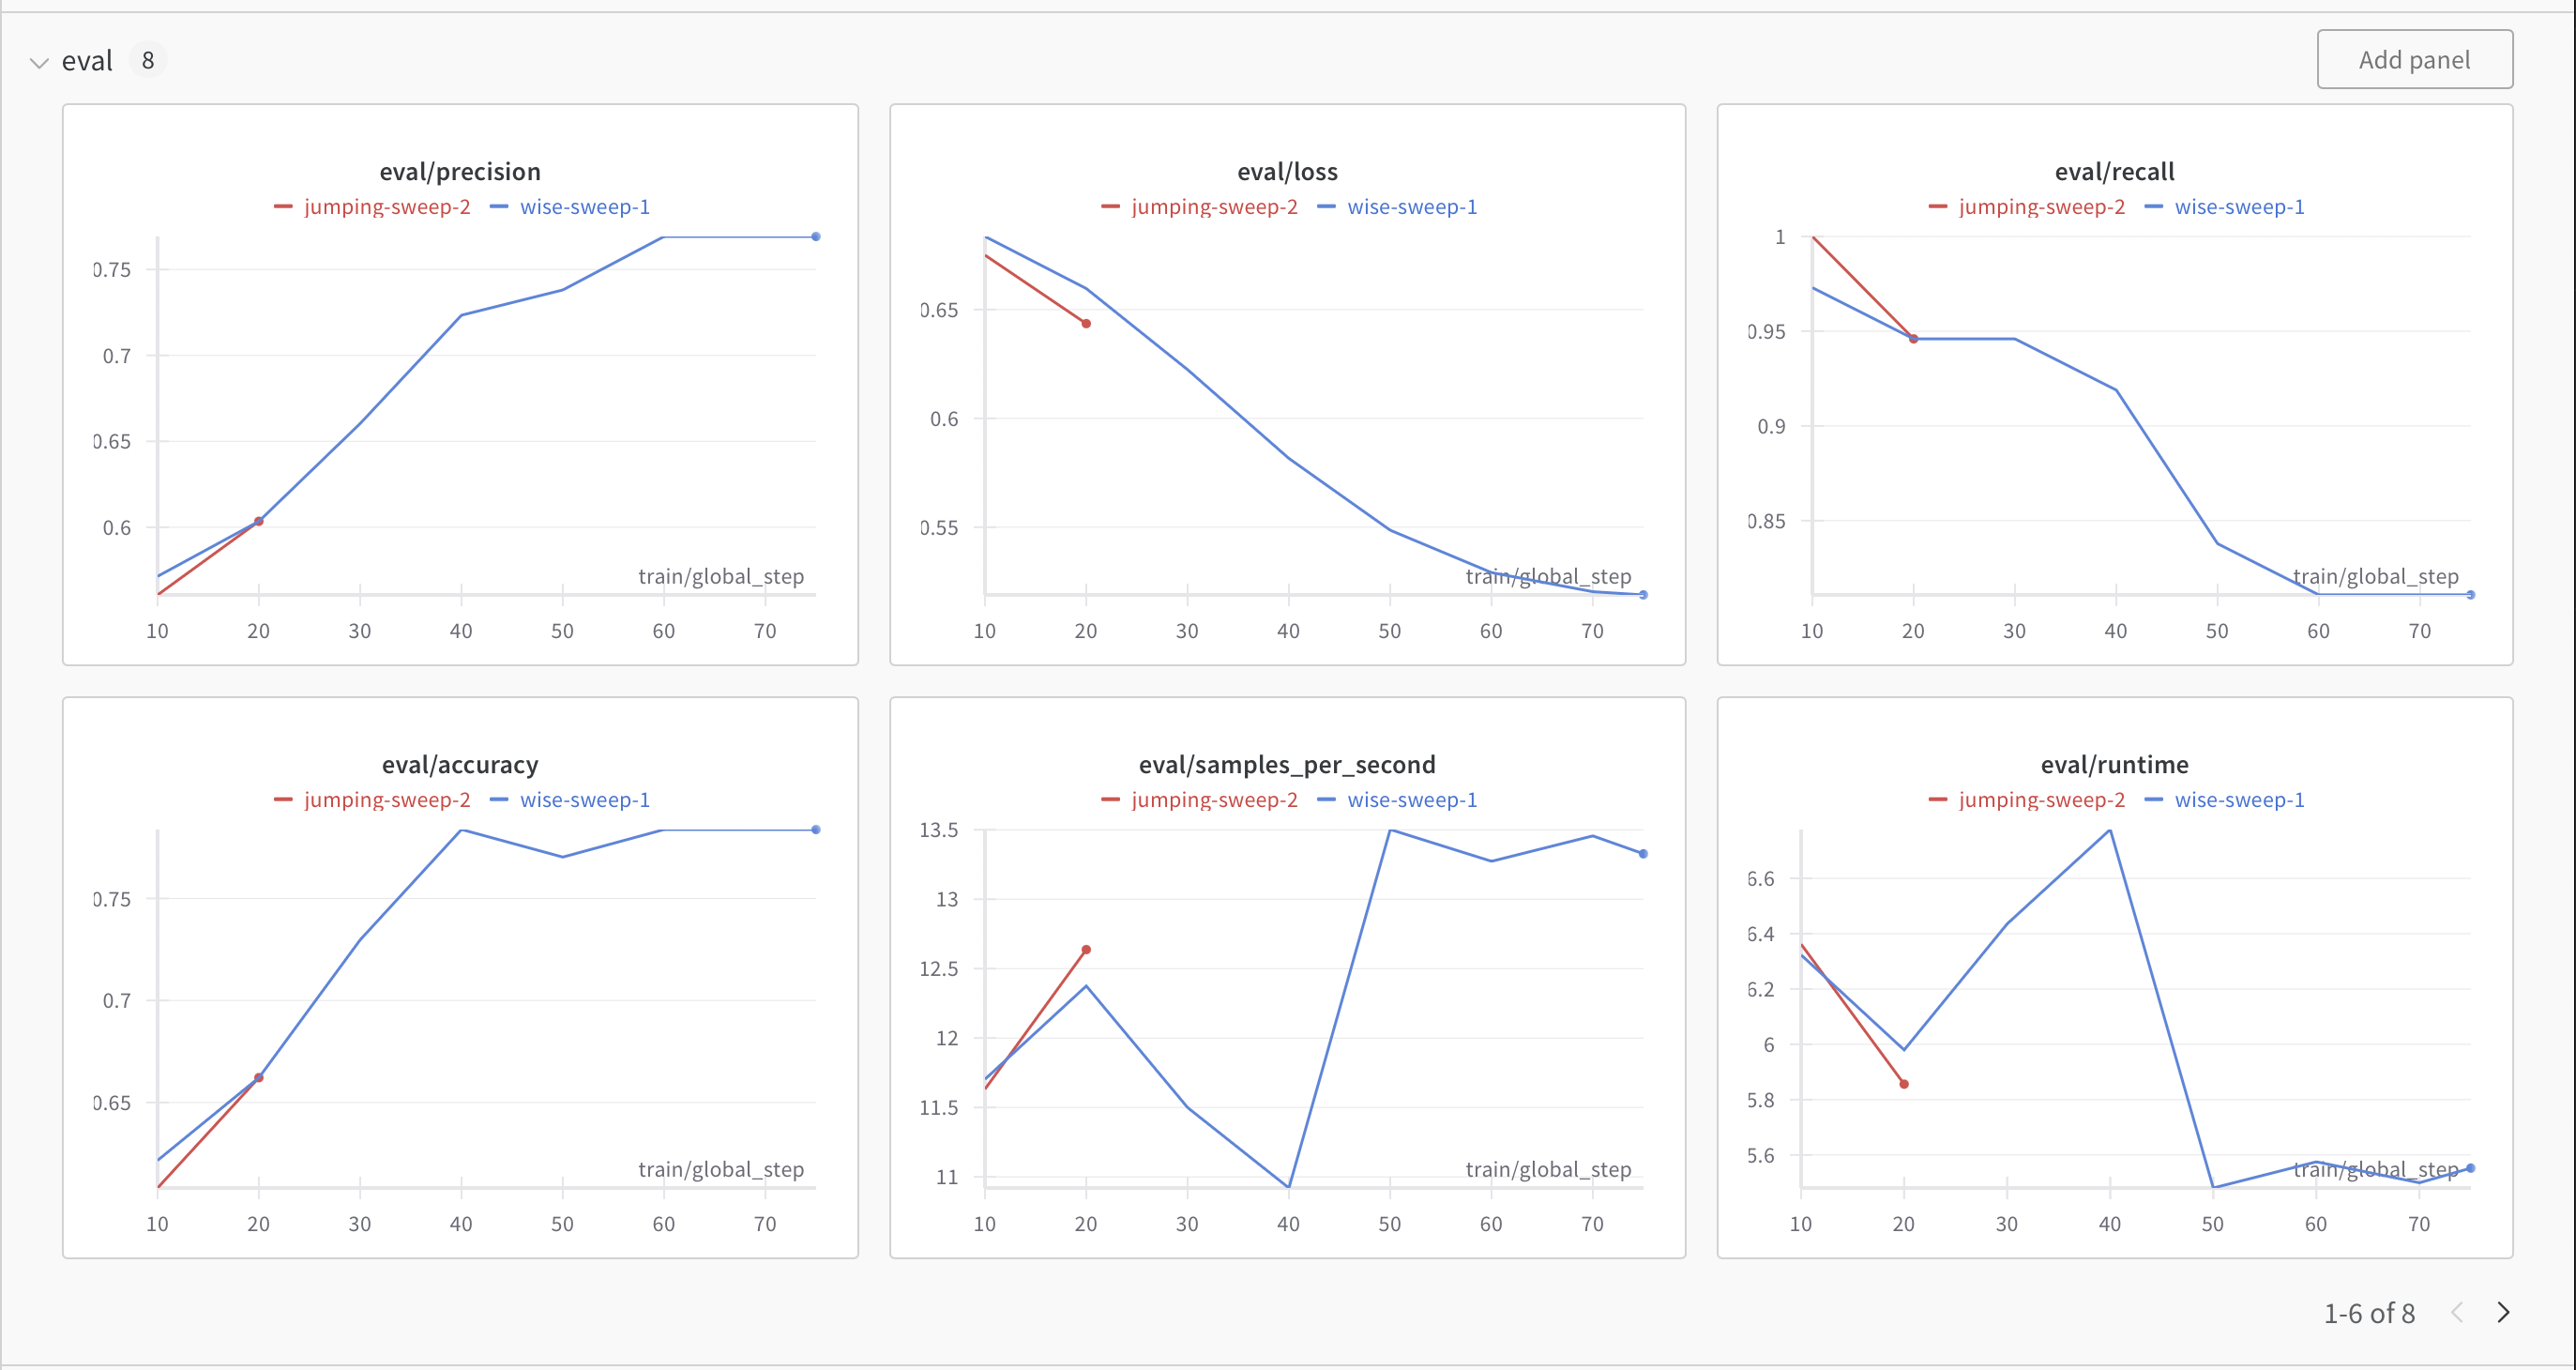
\includegraphics[width=0.7\textwidth]{plots.png}
    \caption{Visualisation des résultats}
    \label{fig:plots}
\end{figure}

La visualisation la plus significative pour notre stratégie de développement du modèle est le "Parallel Coordinates Plot". Cela permet d'examiner les performances de chaque ensemble d'hyperparamètres au cours des itérations du K-Fold, afin de sélectionner les plus efficaces pour réentrainer le modèle et le tester sur un ensemble de Test séparé.

\begin{figure}[!htbp]
    \centering
    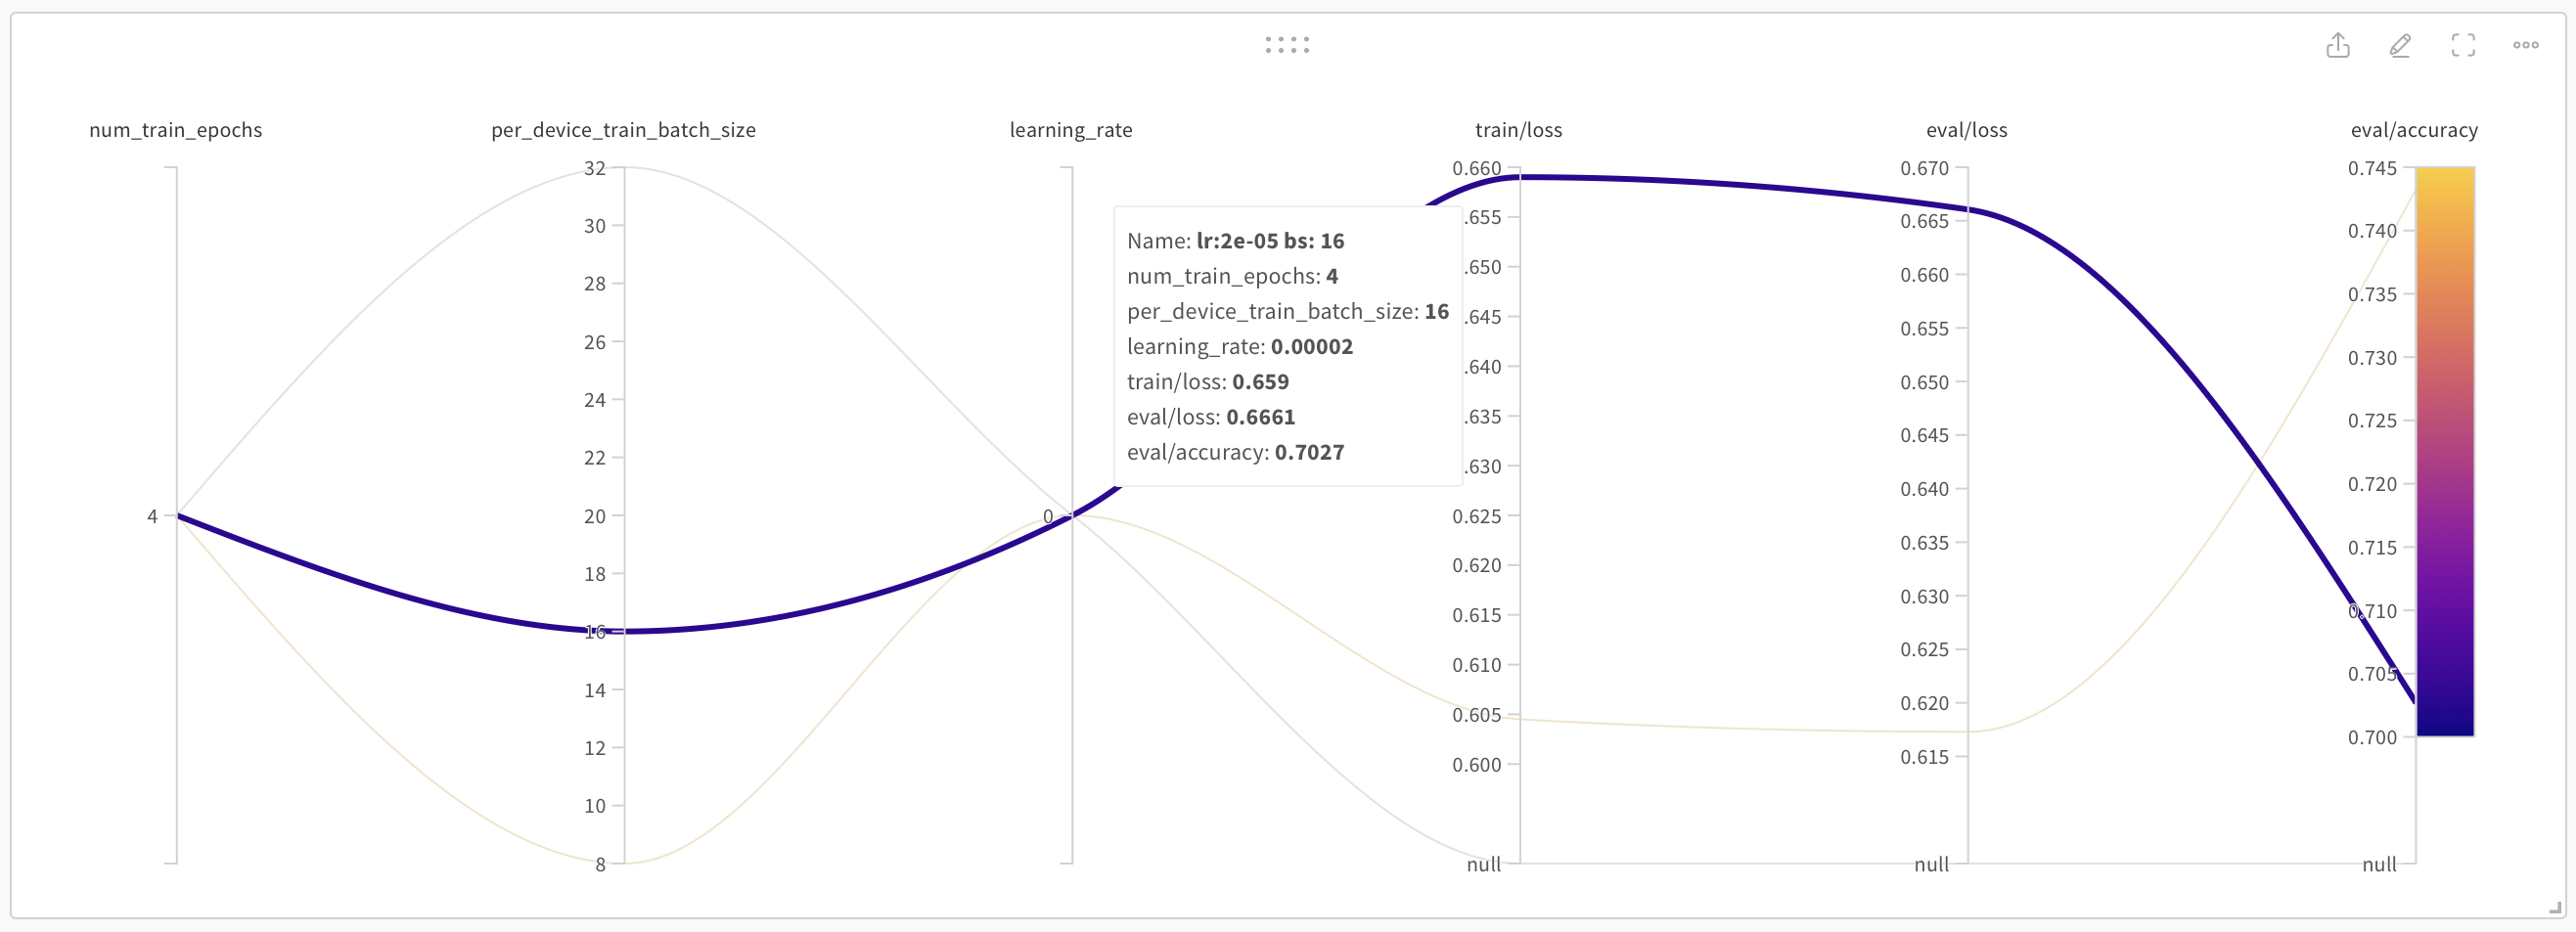
\includegraphics[width=0.9\textwidth]{sweep.png}
    \caption{Parallel Coordinates Plot}
    \label{fig:sweep}
\end{figure}

Pour évaluer les performances sur l'ensemble de Test, WandB offre la possibilité de logger des graphiques classiques de Seaborn et Matplotlib, tels que la courbe ROC et la matrice de confusion. L'ensemble de ces résultats nous permet de tirer des conclusions et de prendre des décisions concernant la capacité de généralisation de notre modèle sur l'ensemble d'entraînement, ainsi que son aptitude à être déployé sur un ensemble de données plus large pour effectuer des prédictions.

\begin{figure}[!htbp]
    \centering
    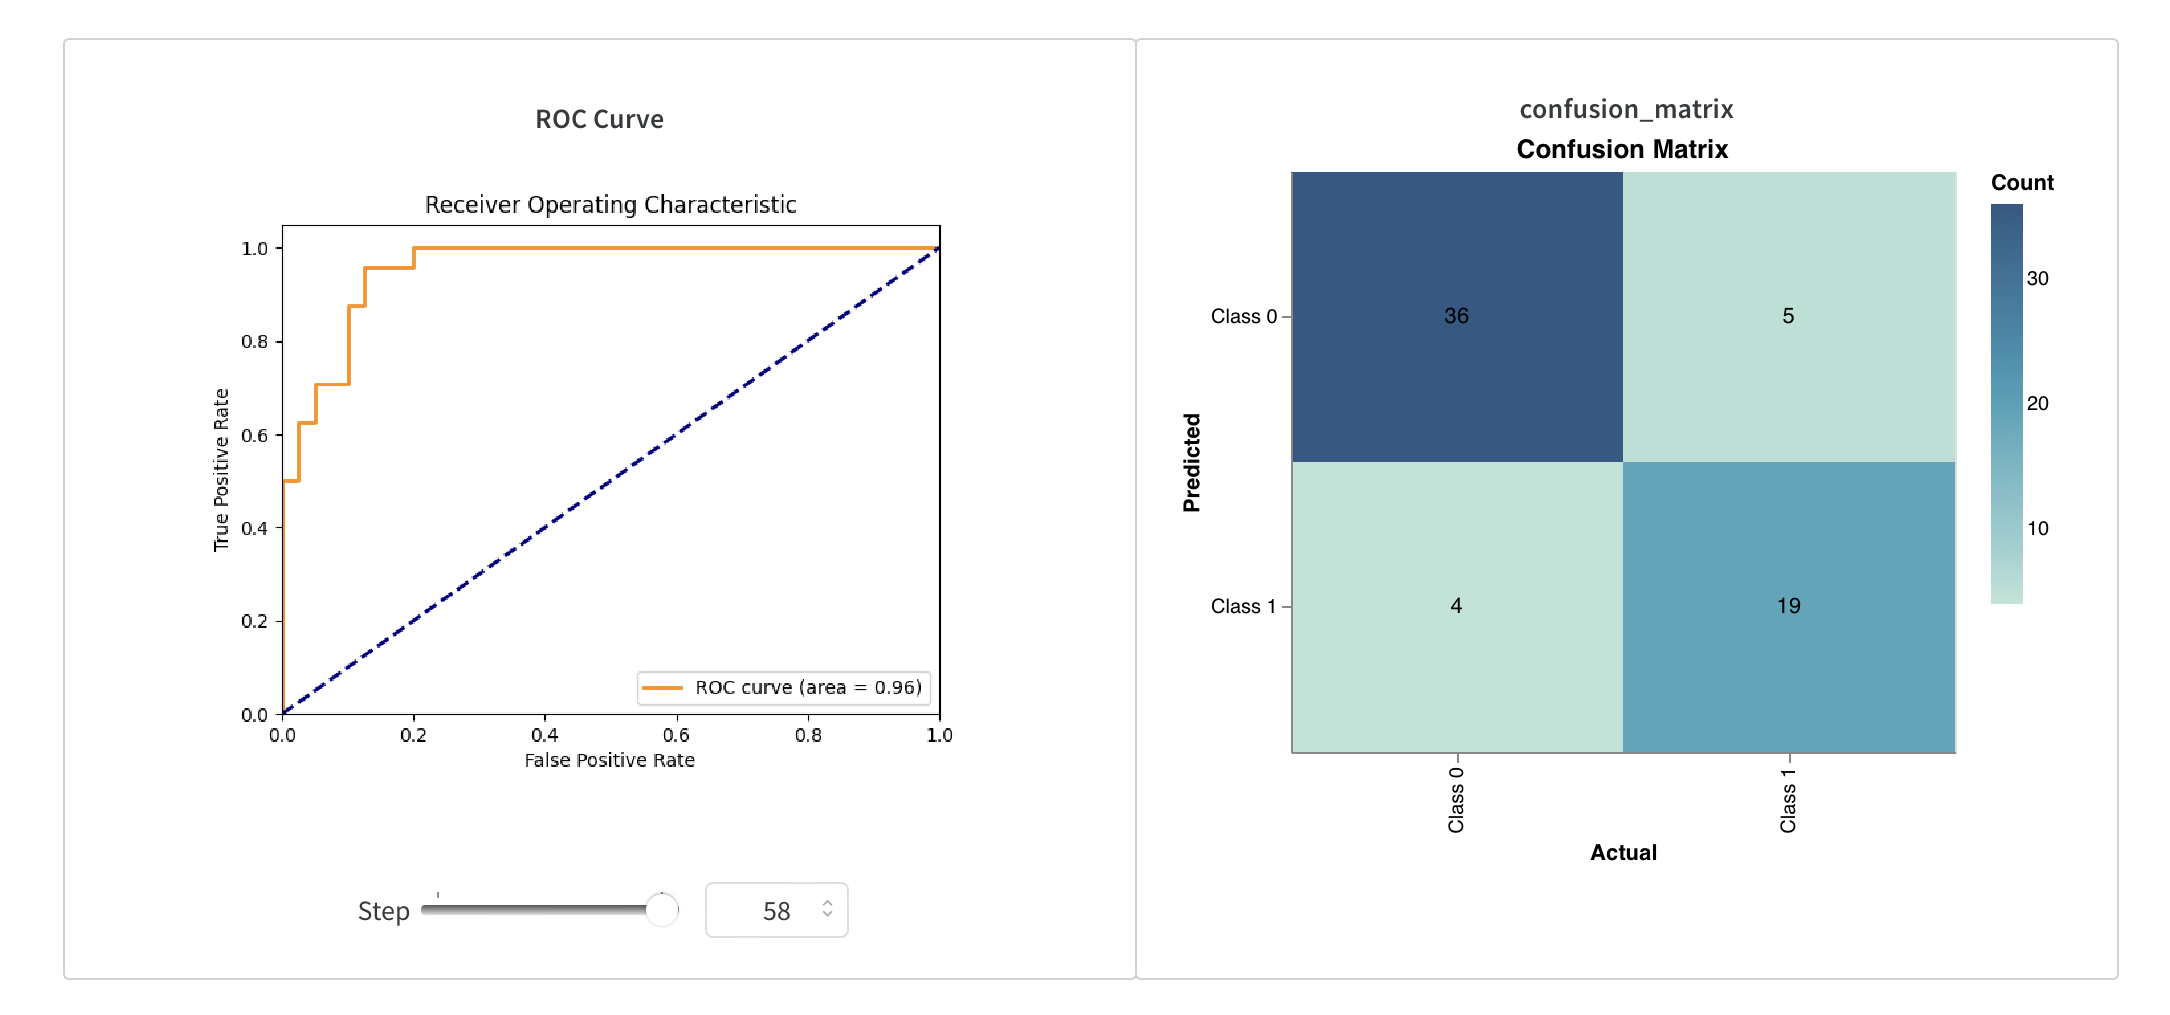
\includegraphics[width=0.7\textwidth]{roc_mtrx.png}
    \caption{La courbe ROC et la matrice de confusion}
    \label{fig:roc_mtrx}
\end{figure}

\section{Clustering}

Les premiers résultats de l'entrainement du modèle de pertinence nous ont permit d'obtenir une liste de 380 articles pertinents à la sécurité alimentaire. Nous avons donc décidé d'effectuer un clustering sur cette liste d'articles. \\

Pour cela, nous avons effectué les étapes suivantes : 
\begin{itemize}
    \item Tokenisation avec CamembertTokenizer
    \item Extraction des caractéristiques
    \item ACP des caractéristiques
    \item Clustering avec un modèle K-means
\end{itemize}

Pour l'ACP, nous avons décidé de conserver 100 composantes afin de préserver 95 \% de la variance expliquée. En utilisant la méthode du coude, nous avons déterminé que le nombre optimal de clusters était de 2, en minimisant la variance intra-cluster.

\begin{figure}[h]
    \centering
    \begin{minipage}{.5\textwidth}
        \centering
        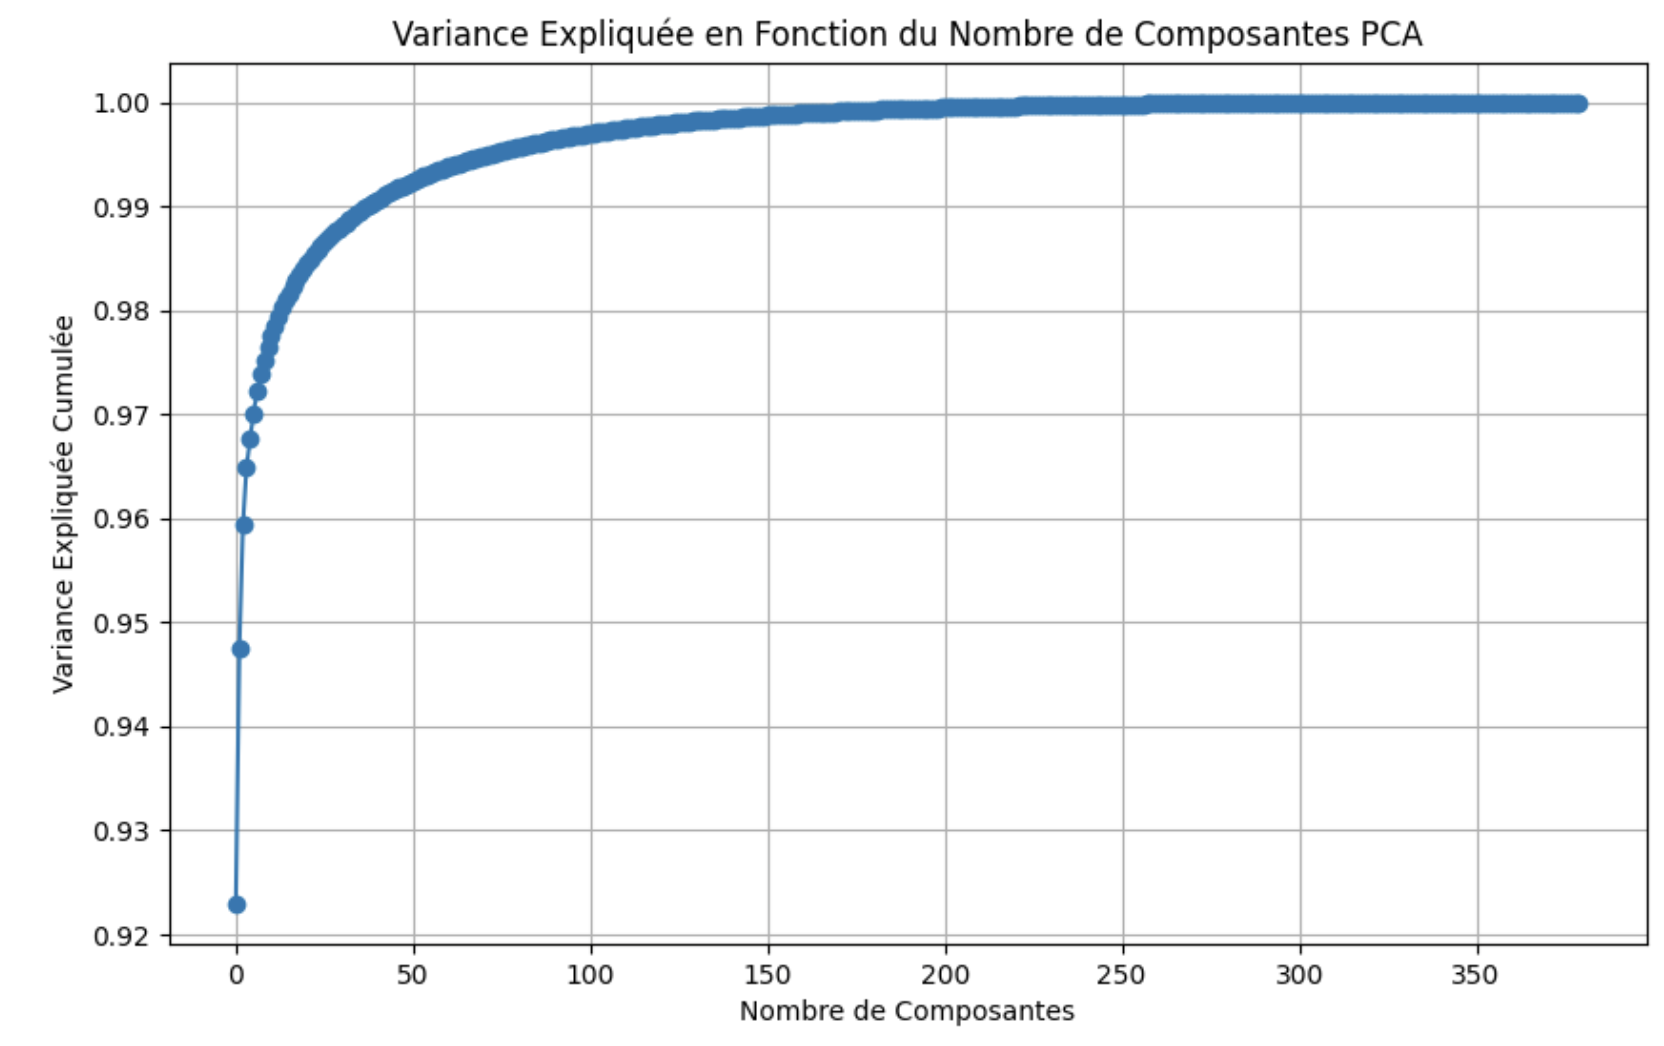
\includegraphics[width=0.75\linewidth]{var.png}
        \label{fig: Variance Expliquée en Fonction du Nombre de Composantes PCA}
    \end{minipage}%
    \begin{minipage}{.5\textwidth}
        \centering
        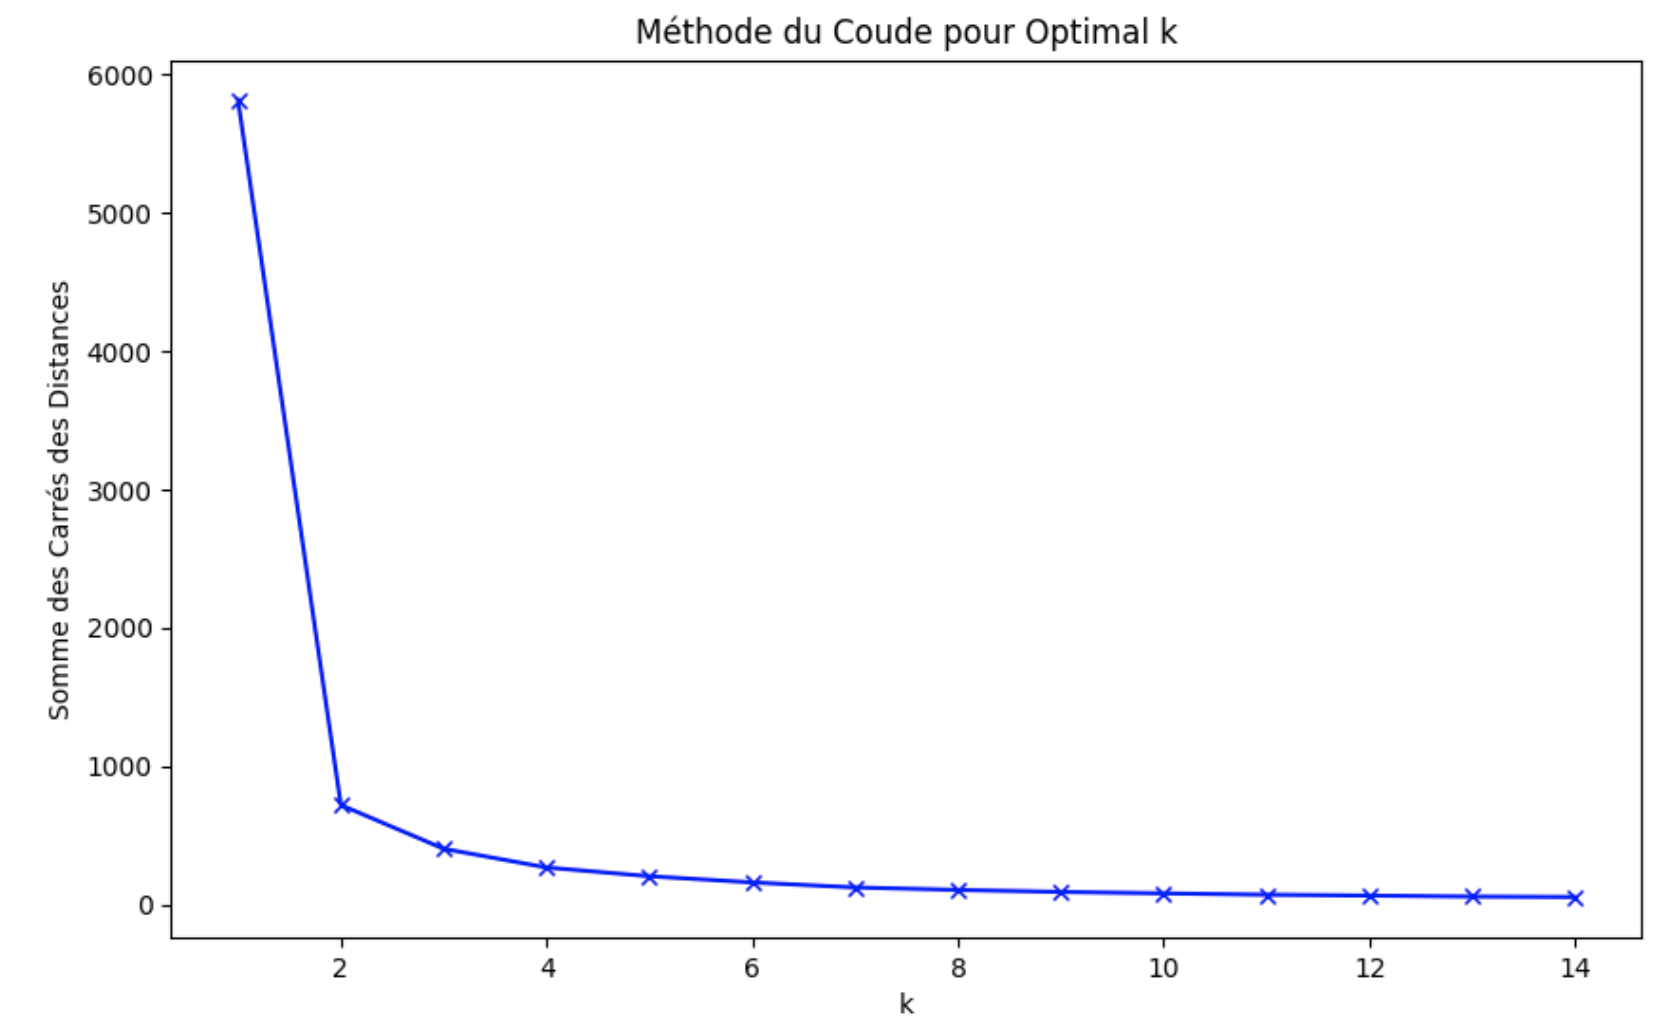
\includegraphics[width=0.8\linewidth]{kopt.png}
        \label{fig: Méthode du Coude}
    \end{minipage}
\end{figure}

\begin{figure}[!htbp]
    \centering
    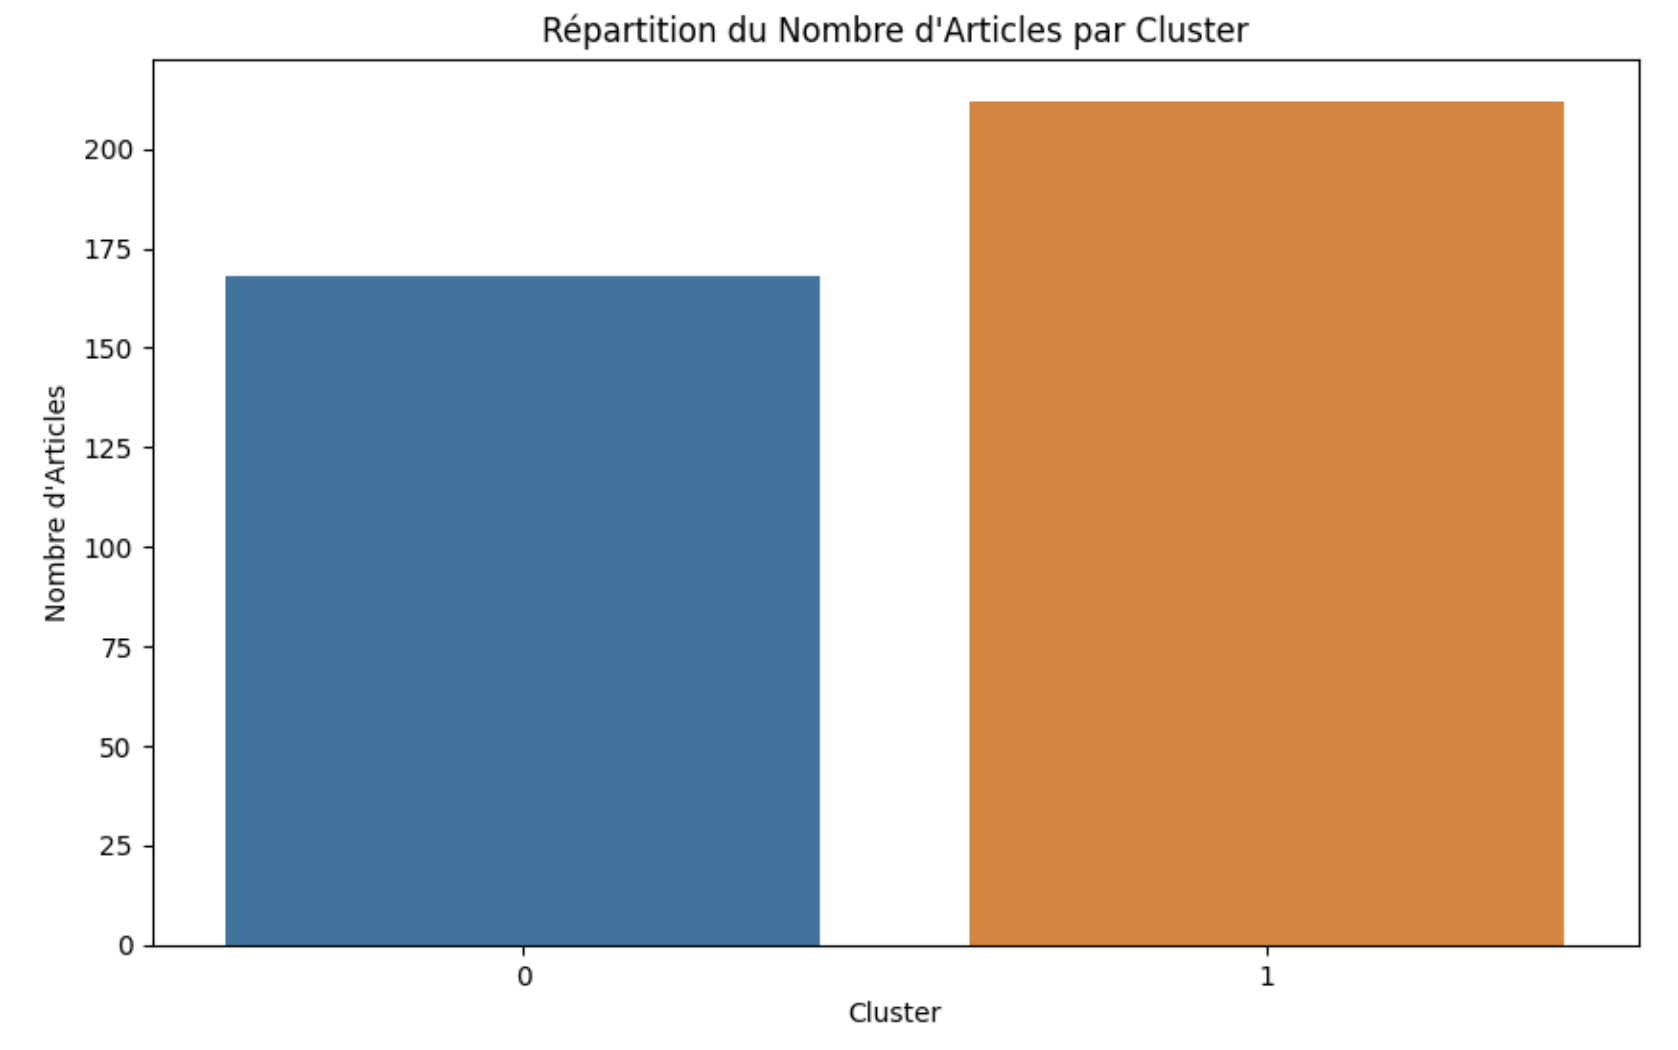
\includegraphics[width=0.4\textwidth]{repart.png}
    \caption{Répartition du Nombre d'Articles par Cluster}
    \label{fig: Répartition du Nombre d'Articles par Cluster}
\end{figure}

Nous avons réalisé une visualisation intéractive permettant de séléctionner les vecteurs de caractéritiques de nos clusters. 

\begin{figure}[h]
    \centering
    \begin{minipage}{.5\textwidth}
        \centering
        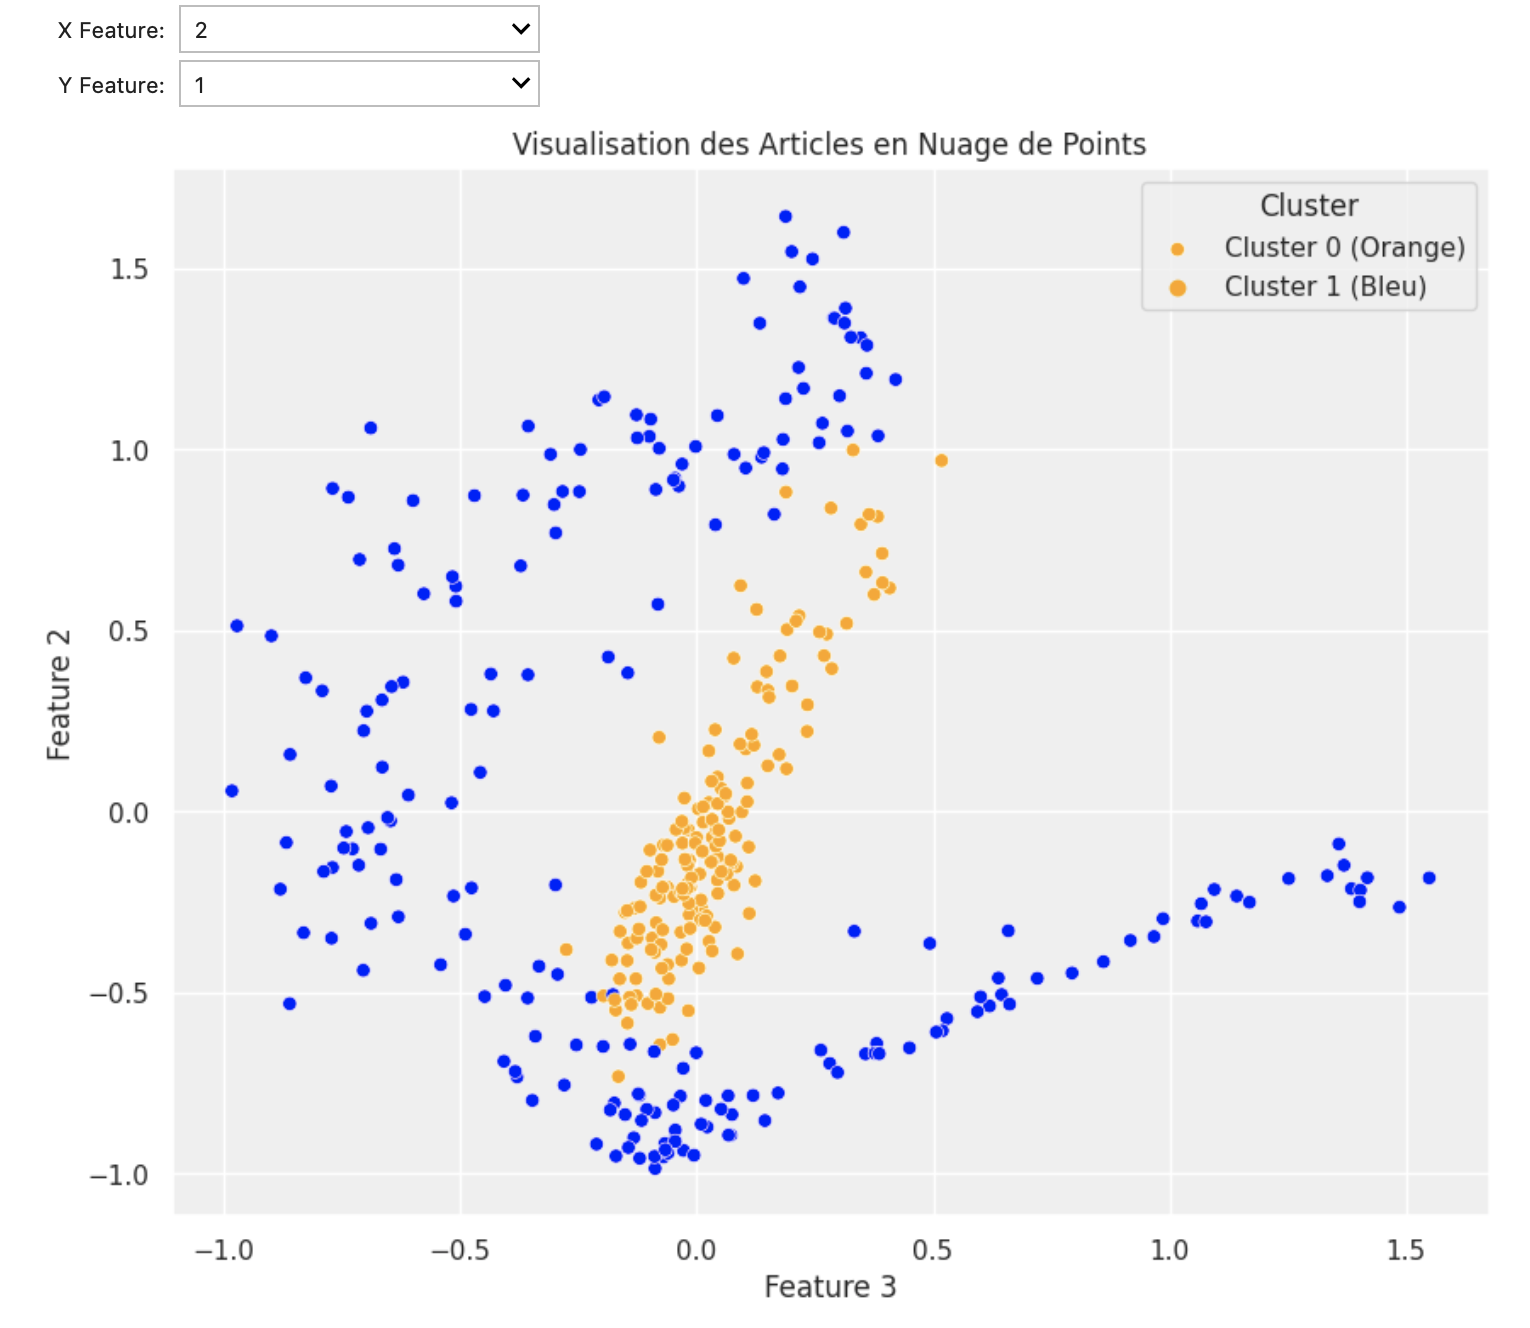
\includegraphics[width=1\linewidth]{visu.png}
    \end{minipage}%
    \begin{minipage}{.5\textwidth}
        \centering
        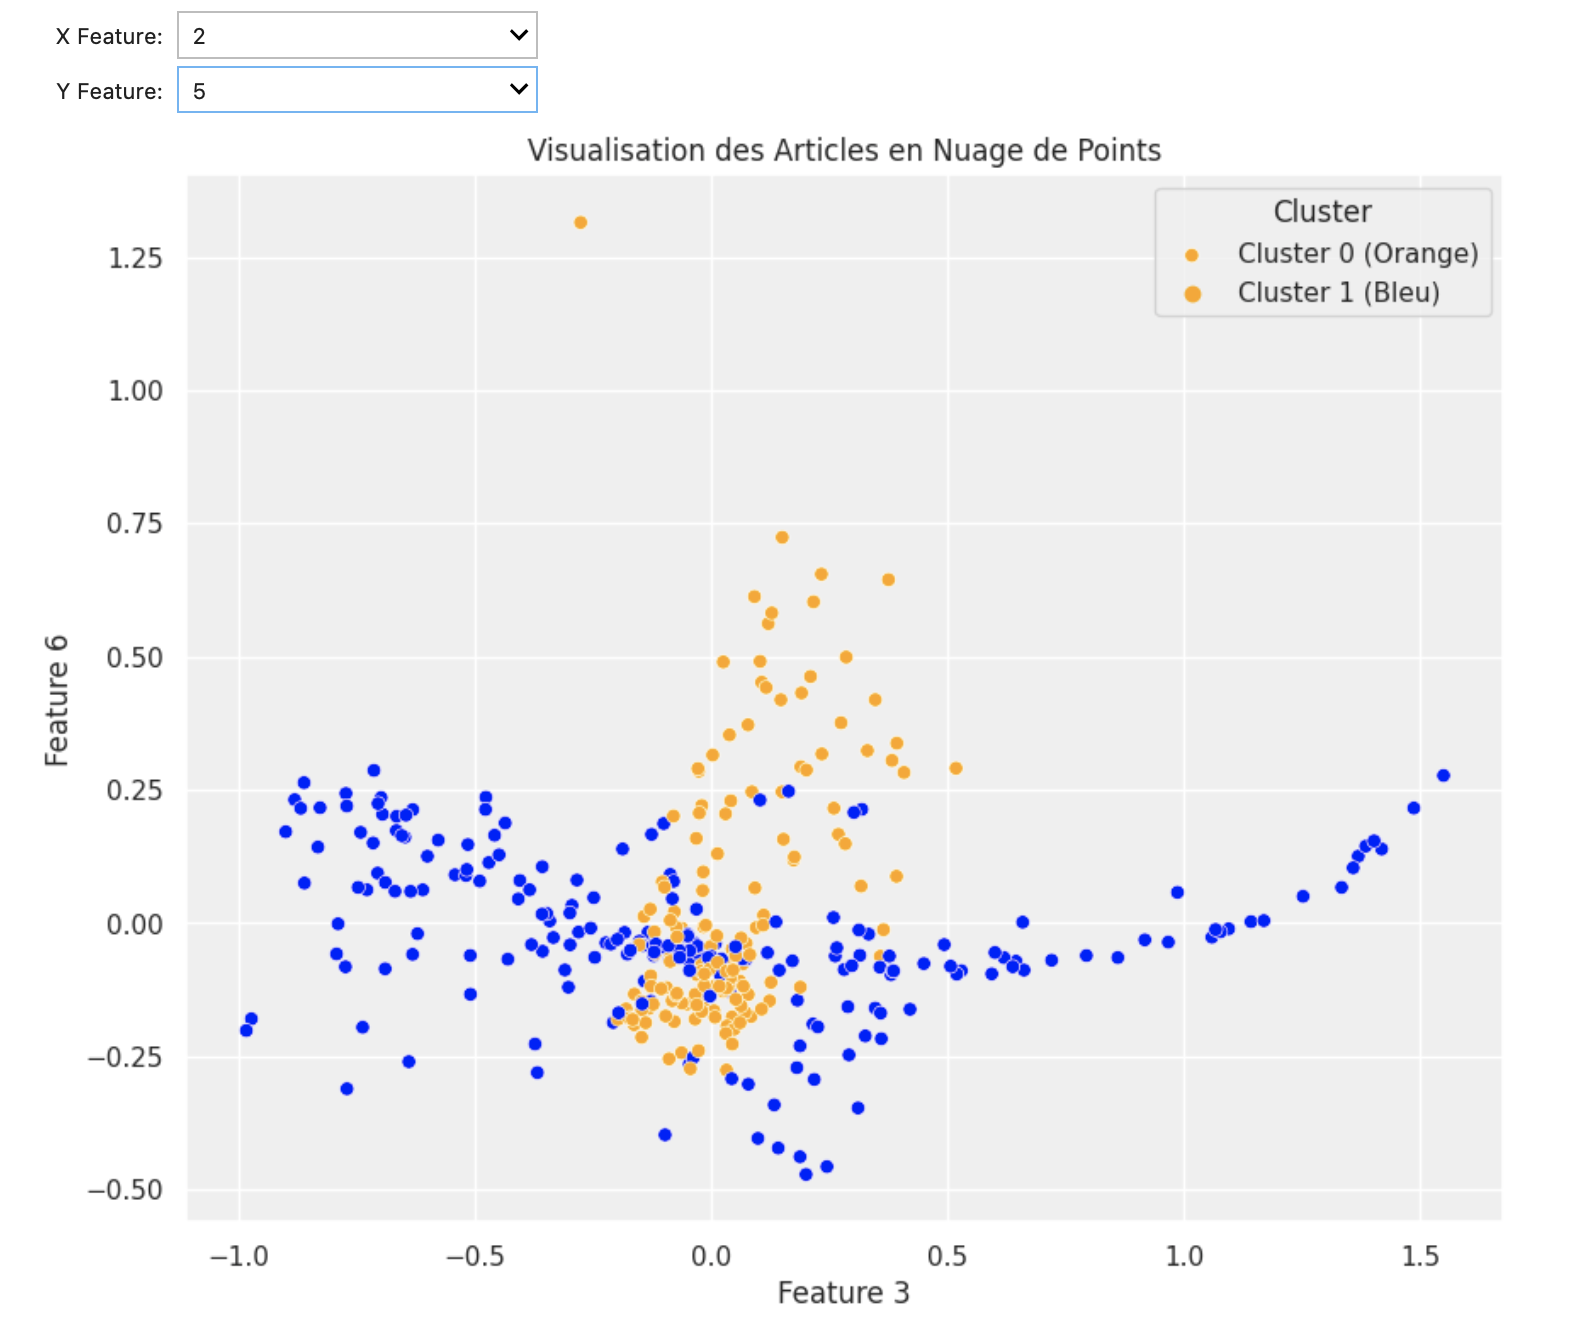
\includegraphics[width=1\linewidth]{visu2.png}
    \end{minipage}
            \caption{Visualisation des Articles en Nuage de Points}
\end{figure}

Dans le rapport dédié à l'interprétation des résultats, nous discuterons de la manière dont nous pouvons interpréter ces clusters de manière plus explicite (article le plus proche du centroïde, identification des mots les plus importants avec TF-IDF).

\section{Cartographie}

Nous avons rencontré plusieurs problèmes concernant la projection de nos articles sur la carte. Le premier concerne l'identification des pays mentionnés dans les articles. Le deuxième problème est que nos articles sont rédigés en français, et par conséquent, les pays mentionnés le sont également, alors que la liste des pays dans GeoPandas est en anglais. \\

Nous avons donc décidé d'extraire manuellement les cinq pays mentionnés dans les articles dans leur ordre d'apparition, en utilisant un prompt avec ChatGPT, en attendant de trouver une solution automatisable. 

\begin{figure}[h]
    \centering
    \begin{minipage}{.5\textwidth}
        \centering
        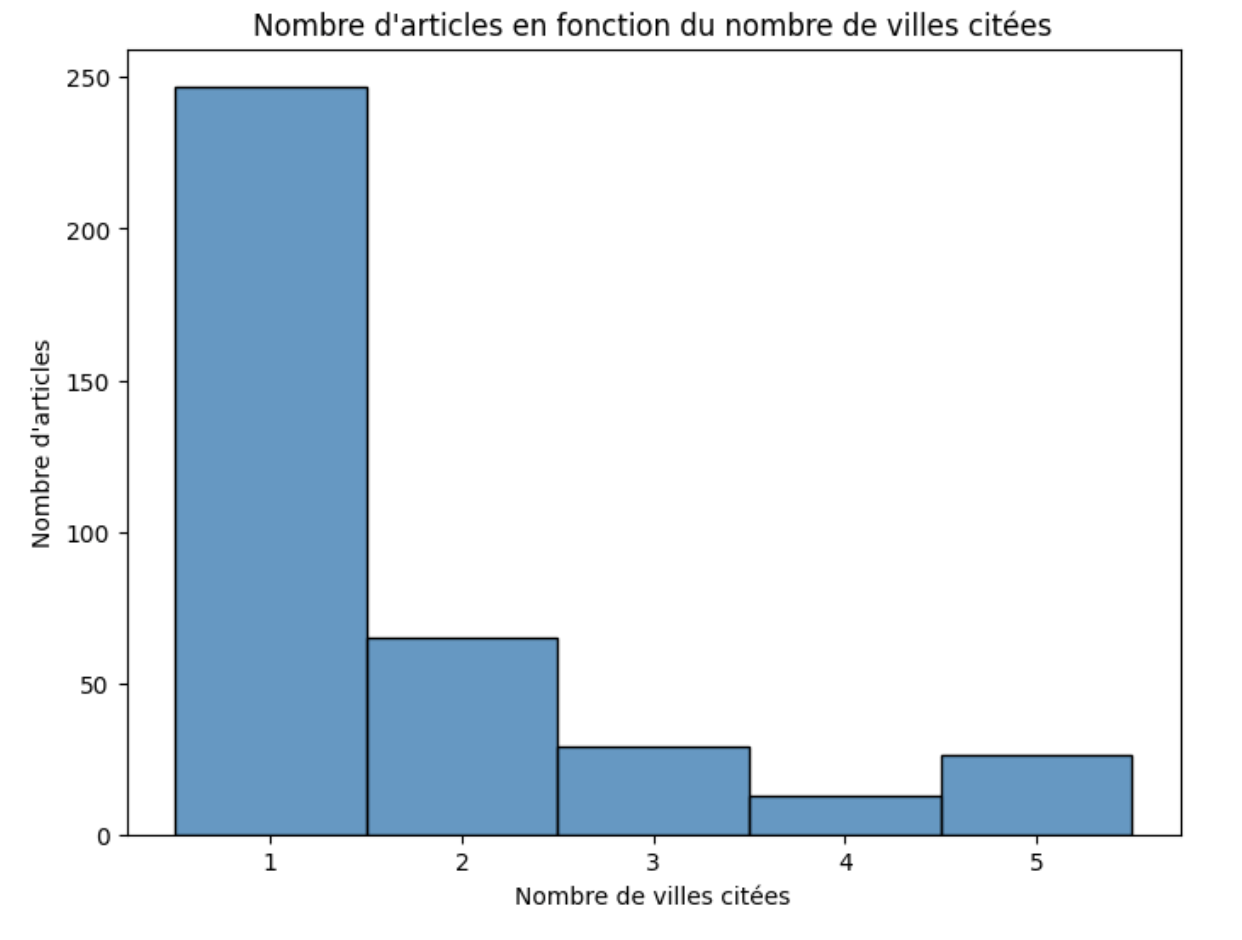
\includegraphics[width=1\linewidth]{nbarticles.png}
            \caption{Nombre d'articles en \\fonction du nombre de villes citées}
    \end{minipage}%
    \begin{minipage}{.5\textwidth}
        \centering
        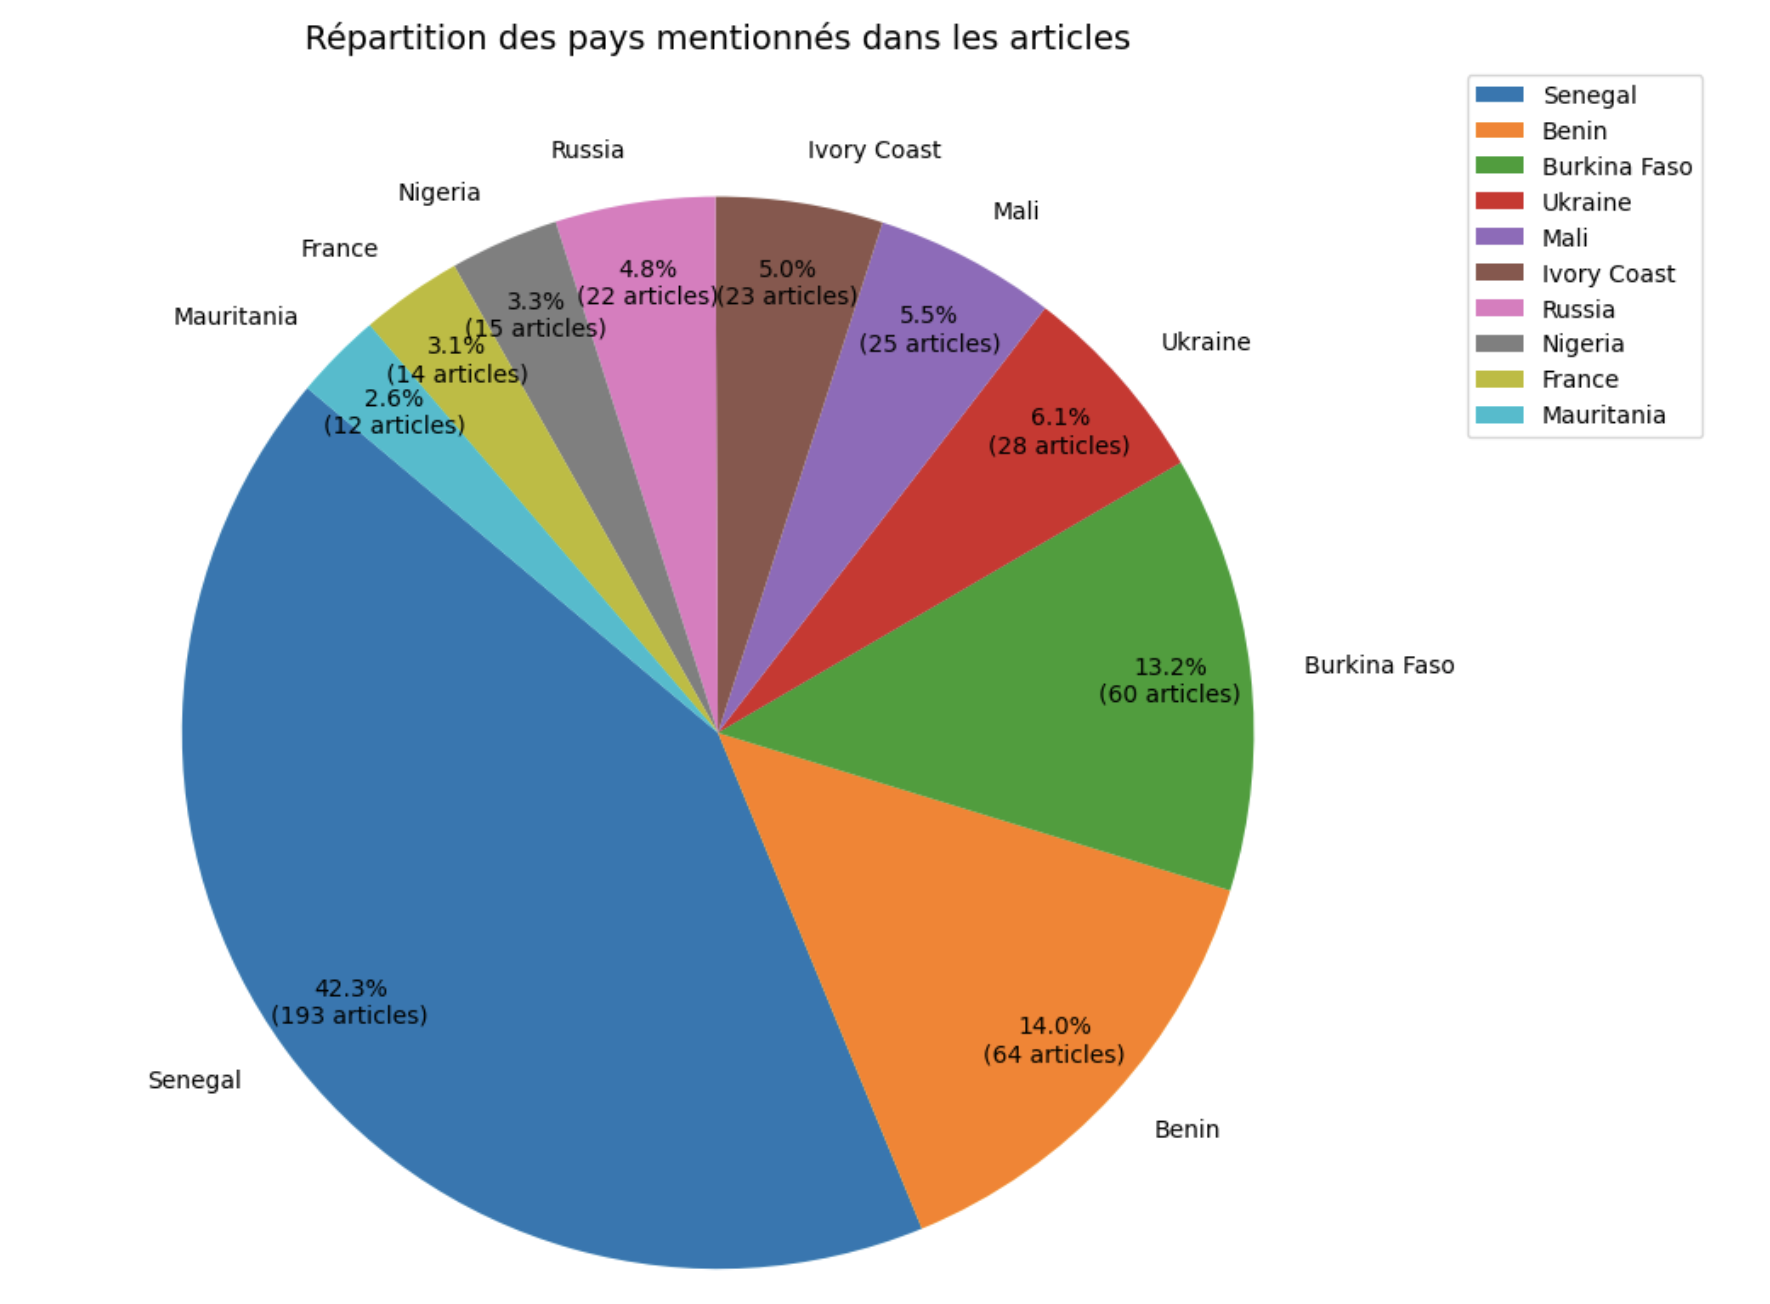
\includegraphics[width=1\linewidth]{Tp10.png}
            \caption{Répartition des pays \\mentionnés dans les articles}
    \end{minipage}
\end{figure}

La majorité des articles (248 sur 380) mentionnent un pays dans leur contenu. Le sénégal, le Bénin et le Burkina faso sont les pays les plus cités. 

\begin{figure}[!htbp]
    \centering
    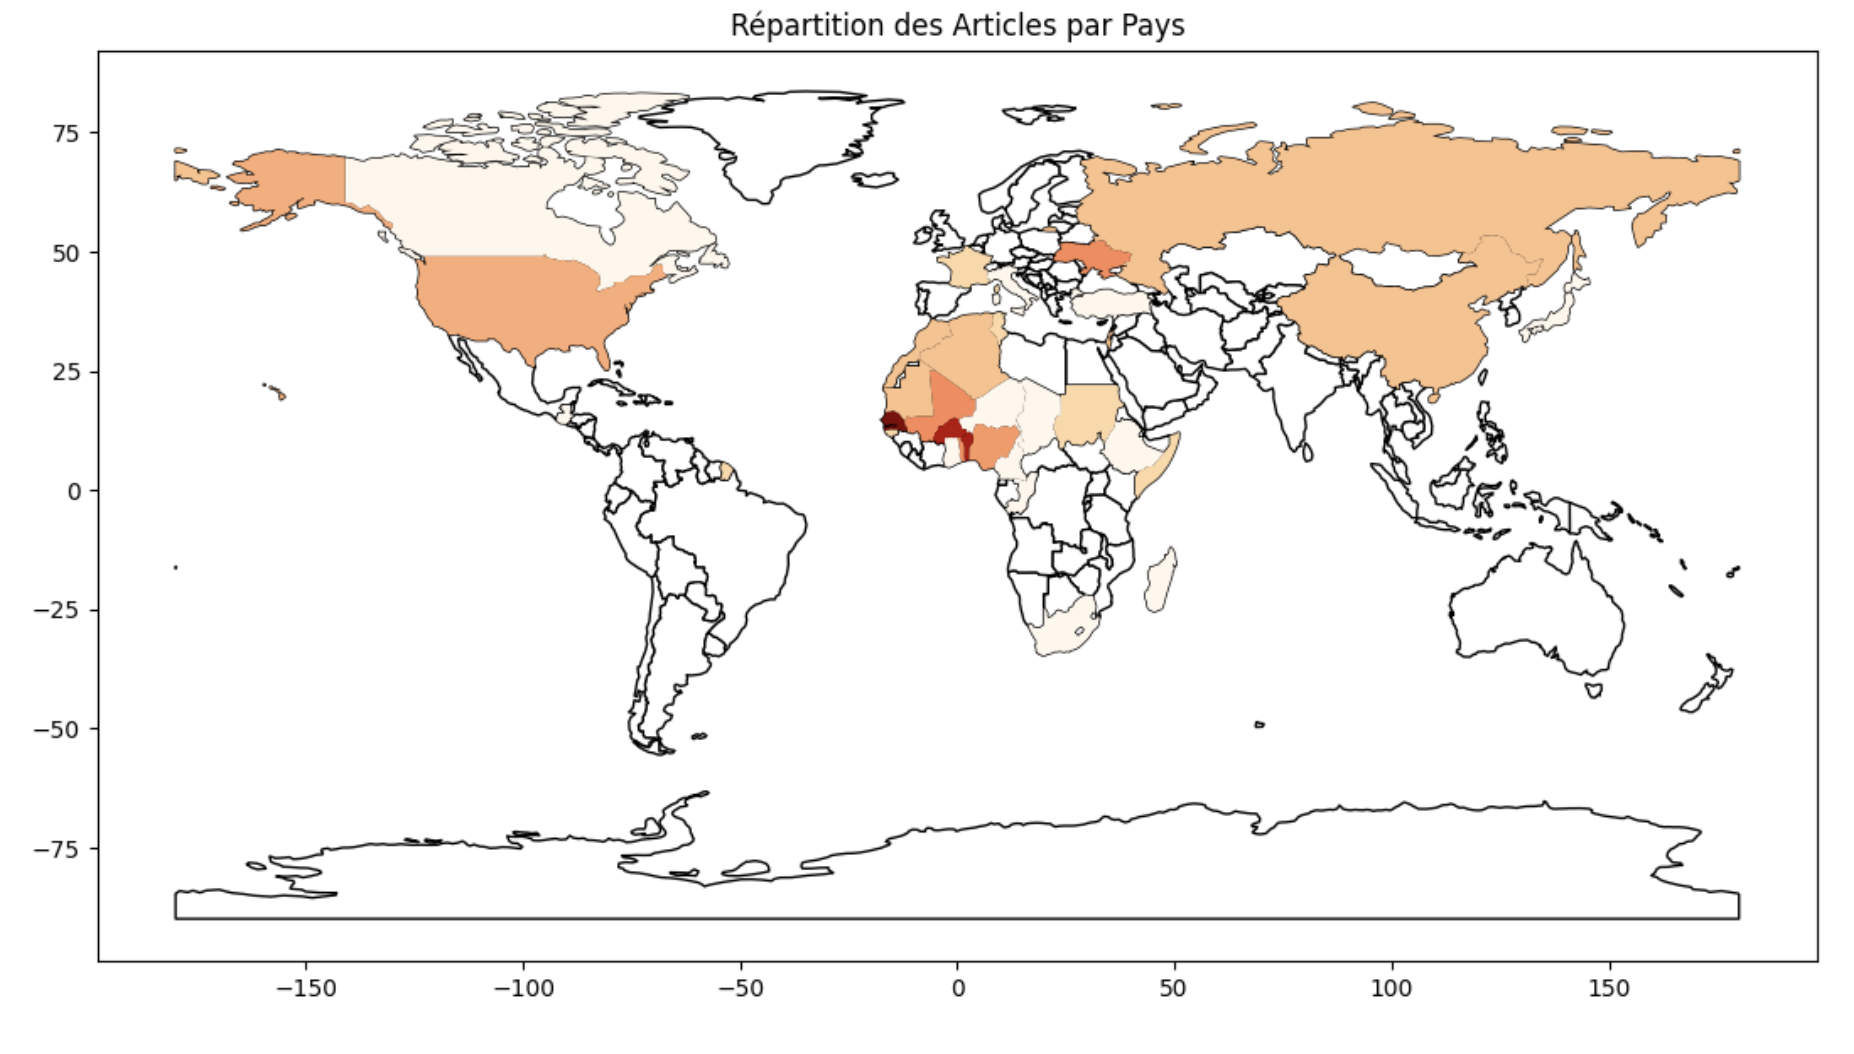
\includegraphics[width=0.8\textwidth]{carte2.png}
    \caption{Répartition des Articles par Pays}
    \label{fig: Répartition des Articles par Pays}
\end{figure}

\section{Conclusions et perspectives}

Notre démarche d'analyses descriptives a permis de mettre en lumière des tendances, comme la baisse de l'indice de négativité au fil du temps et les mots-clés prédominants dans le contexte de la sécurité alimentaire. \\

L'utilisation du modèle BERT ajusté avec l'aide de WandB a amélioré l'efficacité de notre processus de recherche d'hyperparamètres mais a aussi facilité l'interprétation des résultats grâce à des outils de visualisation. \\

L'application de méthodes telles que l'ACP et le clustering K-means sur notre jeu de données a renforcé notre compréhension des 2 groupes au sein des articles pertinents. \\

Pour finir, la cartographie des articles a permis de visualiser la répartition et la fréquence des discussions relatives à la sécurité alimentaire dans différents pays. \\

Nous allons affiner notre modèle de pertinence. Le modèle de clustering ainsi que la carte devront donc être mis à jour. Nous avons l'intention de trouver un moyen moins couteux en temps pour identifier les pays cités au sein de nos articles. La carte devra être intéractive pour permettre à l'utilisateur de cliquer sur un pays et visualiser le nombre d'articles citant ce pays. Nous avons aussi l'intention d'entrainer un modèle d'analyse de sentiment pour produire une carte choroplèthe de la situation des pays en therme de sécurité alimentaire. 

\end{document}
